% FINAL, CHECKED

\chapter{Analýza předchozí práce}\label{ch:analysis}

\chaptersummary{
   \begin{ul}
      \item analýza posudků vedoucího a oponenta předchozí práce,
      \item analýza popsaných možností rozvoje systému,
      \item zkoumání silných a slabých stránek implementovaného systému,
      \item revize změn na fakultě z hlediska správy projektů.
   \end{ul}
}

Tato diplomová práce navazuje na bakalářskou práci z roku 2019~\cite{bachelorthesis} a využívá jak analýzu/výsledky popsané v práci samotné, tak i přílohy (zejména zdrojový kód serverové aplikace, klientské aplikace a vývojářské a uživatelské dokumentace).
Pro implementování daného systému v \g{MSA} a zajištění kvality výsledku je provedena opakovaná analýza problematiky a korekce potřebných oblastí.



\section{Potenciální možnosti rozvoje systému}



\subsection{Posudky}
Ze závěrečných posudků vedoucího a oponenta bakalářské práce je nutno vyčlenit několik významných bodů pro zlepšení.

\begin{ul}
   \item
   \textbf{Neúplná či nedostatečně propracovaná dokumentace~\cite{bachelorthesisreportsupervisor}} – je třeba přepracovat poskytnuté dokumentace a doplnit relevantními informacemi – přidat informace o architektuře, způsobu fungování, zřetelnější práci s databází a použité technologie.
   \clearpage

   \item
   \textbf{Velice stručně popsané testování~\cite{bachelorthesisreportreviewer}} – v poskytnutém systému je velice málo automatizovaných testů a probíhalo zejména manuální testování~\cite{bachelorthesis} – některé části se dají dobře začlenit do vývojového cyklu s automatickým spouštěním.

   \item
   \textbf{Nebylo popsané konkrétní určení informačního systému~\cite{bachelorthesisreportreviewer}} – informační systém od začátku nebyl cílený pro konkrétního spotřebitele.
\end{ul}

Zároveň během obhajoby bakalářské práce bylo nabídnuto zvážit správu a ukládání projektu ve \g{VCS} git místo manuálního ukládání v NoSQL databázi (MongoDB).
To by mohlo zredukovat množství potřebného kódu a snížilo spotřebu fyzické paměti (jednotlivé snímky odevzdaných projektů by se neduplikovaly, ale ukládaly jako git značky\footnote{git tags}).



\subsection{Možnosti rozvoje}

Bakalářská práce navrhuje rozvoj 2 hlavními směry - obecné univerzální zdokonalování a rozvoj se zaměřením na \g{FIT} \g{ČVUT}~\cite{bachelorthesis}.
Jelikož daná práce se soustředí především na \g{MSA}, tak rozvoj se zaměřením na fakultu bude považován za sekundární.
V předchozí práci bylo nabídnuto několik bodů pro rozvoj~\cite{bachelorthesis}.


\begin{ul}
   \item
   \textbf{Podpora internacionalizace a lokalizace} – aplikace poskytuje pouze anglické rozhraní.
   Nepoužívá se žádný framework nebo knihovna, která by napomáhala snadné správě překladů.

   \item
   \textbf{Hromadné zakládání projektů} – neexistuje způsob hromadného zakládání projektů, i když dle předchozí analýzy by byl prospěšný.

   \item
   \textbf{Serverová implementace snímků} – nedokončená funkcionalita pro odevzdávání jednotlivých iterací projektů.

   \item
   \textbf{Nepříznivé scénáře \g{API} dotazů} – v případě pádu serveru a neočekávané \g{API} odpovědi často chybí uživatelsky přijatelné oznámení/zpracování.

   \item
   \textbf{Nové interprety obsahu} – jedná se o omezený výběr vytvářených typů obsahů.

   \item
   \textbf{Propracovaná integrace se službami třetích stran} – funkcionalita propojení fakultních služeb pro známkování, autorizaci apod.

   \item
   \textbf{Analýza využití systému a aktualizace \g{UX}} – bez produkčního prostředí (nebo jiného dlouhodobého uživatelského testování) nebylo možné získat daná data.

   \item
   \textbf{Optimalizace stávajícího systému} – různorodá optimalizace předchozího \g{IS}.
\end{ul}



\subsection{Revize kódu}

\begin{ul}
   \item
   \textbf{\g{IS} není plně kontejnerizovaný} – \g{IS} není plně převeden na kontejnery, může být zdlouhavější start projektu, to se v pozdějších fázích odrazí i na předpokládané škálovatelnosti služby.

   \item
   \textbf{Monolitická struktura aplikace} – jakákoliv úprava vyžaduje editaci celého systému, není možné pohodlně měnit jednotlivé části aplikace.

   \item
   \textbf{Staré a vyřazené z provozu knihovny} – v klientské React aplikaci se nachází starší knihovny, jež musí být aktualizovány (bezpečnost, nová funkcionalita, \dots).
   Rovněž je možné uplatnit nový způsob psaní React aplikací – s React Hooks.

   \item
   \textbf{Konfigurace a zbytečné oddělování prostředí} – bude potřeba zvážit konfiguraci přes \texttt{.env} soubory a odstranit rozdělení způsobů startu aplikace dle prostředí.

   \item
   \textbf{Struktura projektu, architektura} – některé prvky, struktura složek a návrh architektury se zdají být v mnoha případech zbytečné a přispívají nečitelnosti.
\end{ul}



\section{Silné stránky}
Z hlediska pozitivních prvků poskytnuté implementace lze vytknout několik skutečností:

\begin{ul}
   \item
   \textbf{JavaScript, TypeScript a Node.js} – serverová a klientská část aplikace jsou psány v jazyce JavaScript (případně TypeScript), je to výhodné z hlediska udržování systému.

   \item
   \textbf{Knihovna Next.js} – klientská část je psána v jedné z moderních knihoven Next.js s podporou \g{SSR} a \g{SSG}~\cite{nextjs}.

   \item
   \textbf{Dynamicky generovaný obsah projektů} – způsob tvorby obsahu stránky připomíná implementaci mikroslužeb na straně klienta.

   \item
   \textbf{Kontejnerizace aplikací} – databáze jsou poskytovány s pomocí služby Docker a potřebují minimum konfigurací.
\end{ul}



\section{Alternativní systémy správy projektů na fakultě}

Vzhledem k relativně dlouhé době (3 roky) od dokončení bakalářské práce je potřeba provést stručnou aktualizaci seznamů alternativních řešení pro správu projektů na fakultě.
U předchozích systémů fungujících na fakultě (v návaznosti na rešerši způsobů správy projektů na \g{FIT} \g{ČVUT}~\cite{bachelorthesis}) je možné zaznamenat následující změny:

\begin{ul}
   \item
   \textbf{Project/SwinPro} – provoz aplikace je ukončen ke dni 1. 10. 2021 a veškerá data jsou dostupná pouze na požádání prostřednictvím osobního e–mailu~\cite{swinpro}.
   \item
   \textbf{Roundcube\footnote{Webmail}} – byl nahrazen službou Microsoft 365 s vlastními e–mailovými schránkami~\cite{emailsfitcvut}.
   \item
   \textbf{Microsoft Teams} – během vzdálené výuky některé předměty využily funkcionality služby Microsoft Teams pro vytvoření požadavku na odevzdání souboru semestrální práce\footnote{Jedná se o osobní zkušenost z předmětů NI–MPI a NI–PIS}.
   \item
   \textbf{Studentský odevzdávací systém} – vznikl nový portál pro studentské projekty.
   Jelikož se jedná o komplexní řešení, bude rozebrán samostatně v následující podkapitole.
\end{ul}



\subsection{Studentský odevzdávací systém (SOS)}

\textbf{Autor:} kolektiv autorů (závěrečné práce)\newline
\textbf{Analyzovaná verze:} 0.2.3-alpha\newline
\textbf{Datum analýzy:} 31.~10.~2021\newline
\textbf{URL:} \url{https://sos.fit.cvut.cz/}

\begin{figure}[htbp]
   \centering
   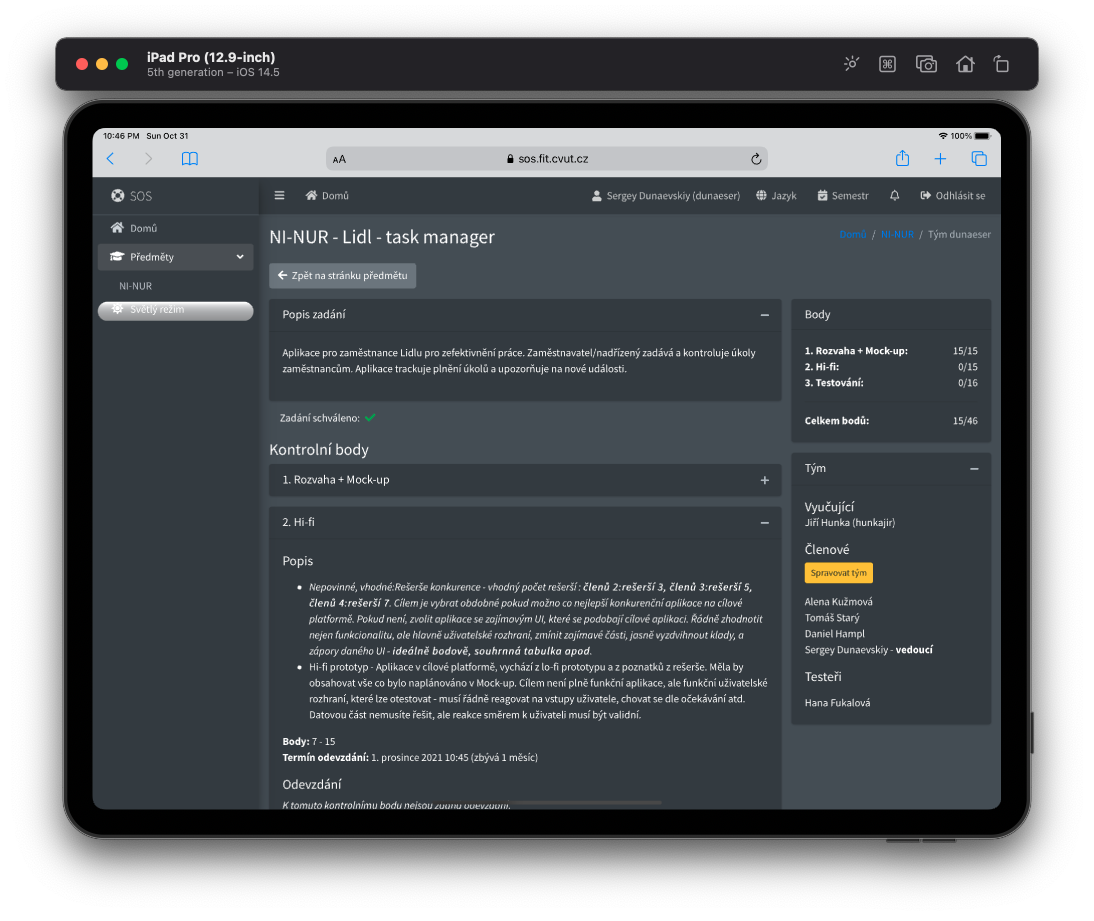
\includegraphics[max width=\textwidth]{assets/analysis-sos-portal}
   \caption[Studentský odevzdávací systém – ukázka detailu projektu]{Studentský odevzdávací systém – ukázka detailu projektu z pohledu studenta}\label{pic:sos-portal}
\end{figure}


Studentský odevzdávací systém je relativně nový portál – nachází se v alpha verzi a využívá se například v předmětu NI-NUR.
Konceptuálně je myšlen jako univerzální systém pro všechny možné projekty, které vyžadují iterativní odevzdávání souborů a obdržení ohodnocení za odevzdanou práci.
Z pohledu studenta lze vytvořit návrh projektu, který může, ale nemusí být schválen vyučujícím, bohužel nelze vytvářet nekontrolované projekty pro vlastní účely.
Následuje tvorba projektu mimo systém a odevzdávání výsledků v podobě samostatných souborů s případným komentářem.
Započatý projekt nelze přerušit ze strany studenta.
Daný systém se v mnoha ohledech podobá \g{IS}, který byl analyzován v předchozích podkapitolách.

\textbf{Společné rysy}

\begin{ul}
   \item
   \textbf{Iterativní odevzdávání projektu} – založený projekt se odevzdává v iteracích (kontrolních bodech), které mohou být okomentovány a ohodnoceny ze strany vyučujícího.
   \item
   \textbf{Odpovědná osoba} – existuje role (vyučující), která dokáže ohodnotit kontrolní bod určitých počtem bodů.
\end{ul}


\textbf{Výhodné prvky}

\begin{ul}
   \item
   \textbf{Nahrávání souborů} – v rámci iterace lze nahrávat libovolné soubory.
   \item
   \textbf{Integrace s fakultními systémy} – \g{IS} je víc přizpůsobený pro fakultní účely.
   \item
   \textbf{Tmavé rozhraní} – \g{UI} má volitelný tmavý režim, viz obrázek~\ref{pic:sos-portal}.
   \item
   \textbf{Jazyky} – \g{UI} je poskytováno v anglickém a českém jazyku s libovolným přepínáním.
\end{ul}


\textbf{Negativní prvky}

\begin{ul}
   \item
   \textbf{Restrikce zakládání projektů} – studenti nemohou zakládat vlastní, nezávislé projekty, musí spadat pod určitý předmět.
   Nelze založit a spravovat víc projektů.
   \item
   \textbf{Nelze založit víc projektových rolí} – projektové role i pro vedoucího projektu jsou omezeny na členy týmu a testery, nelze přidat libovolnou roli.
   \item
   \textbf{Neintuitivní rozhraní} – některé prvky uživatelského rozhraní nejsou intuitivně pochopitelné (subjektivně) a při kritické změně nevyžadují potvrzení.
\end{ul}
